\documentclass[a4paper, 12pt,oneside]{article} 
%\documentclass[a4paper, 12pt,oneside,draft]{article} 
\usepackage{preamble_bis}
%--------------------- ACTUAL FILE ---------------------- %
\begin{document} 
%%%
	\begin{titlepage}
    \newcommand{\HRule}{\rule{\linewidth}{0.5mm}} % Defines a new command for the horizontal lines, change thickness here
    
    \center  % Center everything on the page
     
    %----------------------------------------------------------------------------------------
    %   HEADING SECTIONS
    %----------------------------------------------------------------------------------------
    
    \vspace{3cm}
    \textsc{\LARGE École polytechnique fédérale de Lausanne}\\[1.5cm] % Name of your university/college
    
    \textsc{\Large Project N$^\circ$2 Report}\\[0.5cm] % Major heading such as course name
    \textsc{\large Randomized Nystr\"om
    }\\[0.5cm] % Minor heading such as course title
    
    %----------------------------------------------------------------------------------------
    %   TITLE SECTION
    %----------------------------------------------------------------------------------------
    
    \HRule \\[0.4cm] % line above and under the title
    
    
    % Title of your document
    
    \HRule \\[1.5cm]
     
    %----------------------------------------------------------------------------------------
    %   AUTHOR SECTION
    %----------------------------------------------------------------------------------------
    
    \begin{minipage}{0.4\textwidth}
    \begin{flushleft} \large
    
    \emph{Authors:}\\
    Tara \textsc{Fjellman}\\
    Amal \textsc{Seddas}\\
    
    
    
    
    \end{flushleft}
    \end{minipage}
    ~
    \begin{minipage}{0.4\textwidth}
    \begin{flushright} \large
    
    \emph{Professor:} \\
    Laura \textsc{Grigori
     }\\
    \end{flushright}
    \end{minipage}\\[10cm]
    %
    
    
    %----------------------------------------------------------------------------------------
    %   LOGO SECTION
    %----------------------------------------------------------------------------------------
    
    
\includegraphics[width=0.4\linewidth]{Logo-1 .pdf}\\[1cm] 
    % Include a department/university logo - this will require the graphicx package
     
    %----------------------------------------------------------------------------------------
    
    \vfill % Fill the rest of the page with whitespace
    
    \end{titlepage} 
	% Add titlepage
	\clearpage
	\tableofcontents
	\thispagestyle{empty}
	% Add table of contents
	\clearpage
	\pagenumbering{arabic}
	\setcounter{page}{1}

	\section{Introduction}
		\lipsum[1]
	\section{Algorithms}
        \subsection{Sketching Matrices}
        \subsection{Randomized Nyström low rank approximation}
		The goal of this project is to study the randomized Nyström algorithm for computing a rank- $k$ approximation of a matrix $A \in \mathbb{R}^{n \times n}$ that is symmetric positive semidefinite. Given a sketching matrix $\Omega \in \mathbb{R}^{n \times l}$, where $l$ is the sketch dimension, $l>k$, the randomized Nyström approximation relies on the following formula:

		$$
		A_{N y s t}=(A \Omega)\left(\Omega^T A \Omega\right)^{+}\left(\Omega^T A\right)
		$$
		
		where $\left(\Omega^T A \Omega\right)^{+}$denotes the pseudoinverse of $\Omega^T A \Omega$. This formula provides an approximation of $A$ of rank at most $l$. Several solutions are possible for computing a rank-k approximation from $A_{N_{y s t}}$, that we denote as $[A_{N_{y s t}}]_k$. One consists of computing a rank-k decomposition of the matrix $B=\Omega^T A \Omega$, while another one consists of computing a rank-k truncation of the Nyström approximation $A_{N y n t}$. The second approach is considered for this project. Different solutions are proposed in the literature, see one solution in the slides from the lecture on Randomized algorithms for low rank matrix approximation, where the algorithm relies on the Cholesky decomposition or the eigenvalue decomposition of $B$. Other reference is 44]. Two different data sets should be used to validate your considered randomized Nyström low rank approximation, that are described later on. Hence this project should allow you to identify a randomized algorithm that is numerically stable for the considered data sets and scales reasonably well in parallel.
	\section{Data sets}
	We consider two different types of data sets in this project. The first is synthetic and is a part of those described in section 5 of [4]. More precisely, we consider polynomial and exponential decay diagonal matrices with different decay rates, which we call slow, medium and fast in the rest of the report.
	
	The second data set we use  described for example in [1] (section 4). It consists of a similarity matrix build from the MNIST dataset with help of the radial basis function $e^{-\left\|x_i-x_j\right\|^2 / c^2}$. With the first $n$ rows of the MNIST dataset leads to a dense $n\times n$ matrix $A$. The parameter $c$ can be varied to tune how much to penalise dissimilarity. To make the exploration of this value simpler, we decided to first normalize the MNIST dataset by dividing the entries by the maximal intensity across the dataset. 
	
	[ADRESS THIS] The dimension $n$ should be taken depending on what your code can support in terms of memory consumption.
	\section{Stability analysis}
		- bullet points about comments to include 
	\section{Parallelisation}
	We parallelise the algorithm by distributing among the processors the computation of $A \Omega,\Omega^T A \Omega$, and all other matrix operations with complexities at least proportional to $n$. 
	
	The parallelisation of QR factorisation was the topic of the first project. We therefore included the relevant functions for it in the code folder. The parallelisation of matrix products was however implemented from scratch. It was done as 	
	
	$$
	S=\left(\begin{array}{lll}
	S_{0} & S_{01} & S_{02} \\
	S_{10} & S_{11} & S_{12} \\
	S_{20} & S_{21} & S_{22}
	\end{array}\right), \quad \Omega=\left(\begin{array}{l}
	T_0 \\
	T_1 \\
	T_2
	\end{array}\right),
	$$
	with processor $i$ having the $i$-th row of $S$ and the $i$-th block row of $T$. Then

	\begin{algorithm}
		\caption{Computes the matrix product of two matrices $D$ and $E$ in parallel.}
		\begin{algorithmic}
		\Require $q$ is an integer and the square root of the number of processors, $D$ is an $m\times m$ matrix distributed such that processor $i$ has $D_{i//q,i\text{ mod }q}$ and $E$ is a $m\times n$ matrix distributed such that processor $i$ has $E_{i//q}$. FullProd is true if we also want to compute $E^TDE$.
		\Ensure $F=DE$ (and $G=E^TF$ too if FullProd is true). 
		\State $F_{ij} \gets P_{ij}E_j$
		\If{\text{FullProd}}
			\State $G_{ij} \gets E_i^FP_{ij}$
		\EndIf		
		\State Row-wise Sum-reduce : $F_i\gets \sum_j^q F_{ij}$
		\State Column-wise Gather on rank 0 : $F\gets [F_1^T,...,F_q^T]^T$
		\If{\text{FullProd}}
			\State Sum-reduce : $G\gets \sum_{i,j}^{q,q} G_{ij}$
		\EndIf
		%\Comment{Locally on rank 0}
		\end{algorithmic}
	\end{algorithm}
	$A \Omega,\Omega^T A \Omega$ multiplications were implemented 
	The matrix $A$ is distributed among processors by using a two-dimensional block distribution while the matrix $\Omega$ is distributed using a block row distribution. The parallelization of the algorithm is implemented in the following way:
	Describe how you parallelize randomized Nyström and provide pseudo-code of the parallel algorithm. For the parallelization, the matrix $A$ should be distributed among processors by using a two-dimensional block distribution while the matrix $\Omega$ should be distributed using a block row distribution. You can consider that the number of processors is a power of 2 such that you can easily distribute the matrices among processors. For example, when $P=\sqrt{P} \times \sqrt{P}=9$, the matrices $A$ and $\Omega$ are distributed as:



	$$
	B=\Omega^T A \Omega=\left(\begin{array}{lll}
		\Omega_1^T & \Omega_2^T & \Omega_3^T
		\end{array}\right)\left(\begin{array}{lll}
		A_{11} & A_{12} & A_{13} \\
		A_{21} & A_{22} & A_{23} \\
		A_{31} & A_{32} & A_{33}
		\end{array}\right)\left(\begin{array}{l}
		\Omega_1 \\
		\Omega_2 \\
		\Omega_3
		\end{array}\right)
	$$

	\begin{algorithm}
		\caption{Randomized Nystr\"om algorithm. The syntax was adapted from this Overleaf example.}\label{alg:parallel-rand-nystrom}
		\begin{algorithmic}
		\Require $A$ is an $n\times n$ symmetric positive semidefinite matrix, $\Omega$ is a sketching matrix of size $n\times l$, and $k$ is the rank of the approximation
		\Ensure $[A_{N y s t}]_k$, the rank-$k$ randomized Nystr\"om approximation of $A$. 
		\State $C \gets A \Omega$
		\State $B \gets \Omega^T C$
		\State $L, \text{Failed} \gets \text{Cholesky}(B)$ \Comment{Locally on rank 0}
		\If{Failed}
			\State $U, \Lambda \gets \text{EigDecomp}(B)$ \Comment{Locally on rank 0}
			\State $B_k^{+} \gets U(:,1:k) \Lambda(1: k, 1: k)^{+} U(:, 1: k)^T$
			\State $Q, R \gets \text{QR}(C)$ \Comment{Using TSQR}
			\State $\hat{U}_k \gets Q U(:, 1:k)$ \Comment{In parallel}
			\State $[A_{N y s t}]_k \gets \hat{U}_k \Lambda(1: k, 1: k)^{+} \hat{U}_k^T$ \Comment{In parallel}
		\Else{}
			\State $Z \gets C L^{-T}$ \Comment{Computed by substitution : $(LZ^T)^T=C^T$}
			\State $Q, R \gets \text{QR}(Z)$ \Comment{Using TSQR}
			\State $U_k, \Sigma_k, V_k \gets \text{TruncSVD}(R)$
			\State $\hat{U}_k \gets Q U(:, 1:k)$ \Comment{In parallel}
			\State $[A_{N y s t}]_k \gets \hat{U}_k \Sigma^2(1: k, 1: k) \hat{U}_k^T$ \Comment{In parallel}
		\EndIf
		\end{algorithmic}
	\end{algorithm}
	
	\section{Experimental procedure}
		- averaging to increase precision of results
		- when running in parallel, was simited by number of cores $p=2^{2s}$ with $s\in\mathbb{N}$ (due to perfect square constraint of the paralelised matrix multiplication and the SHRT algorithm using the Hadamard transform), so we ran results for 1,4,16,64
		- ran results on the Helvetios cluster 
		- $k$ was taken often around $n/20$ as we deemed this value relevant for real applications
		- n was made vary as powers of $2$ due to the Hadamard transformation while $l$ was taken logaritmically spaced just to make the visuals more easy to interpret  
	\section{Algorithm Performance}
        \subsection{Sequential Performance}
		- in general (both plots) observe that k rank approximation represents minority of runtime (as expected as of order $k^3 +nk^2$). Indeed for shown examples represents at most 10\%. This would be different if one were to take big values of $k$. Also does not really seem to depend on sketching method which makes sense given the computations are the same regardless of which sketching method was used to obtain the B and C matrices
		\begin{figure}[htb]       
			\centering             
				\vspace{0em}
				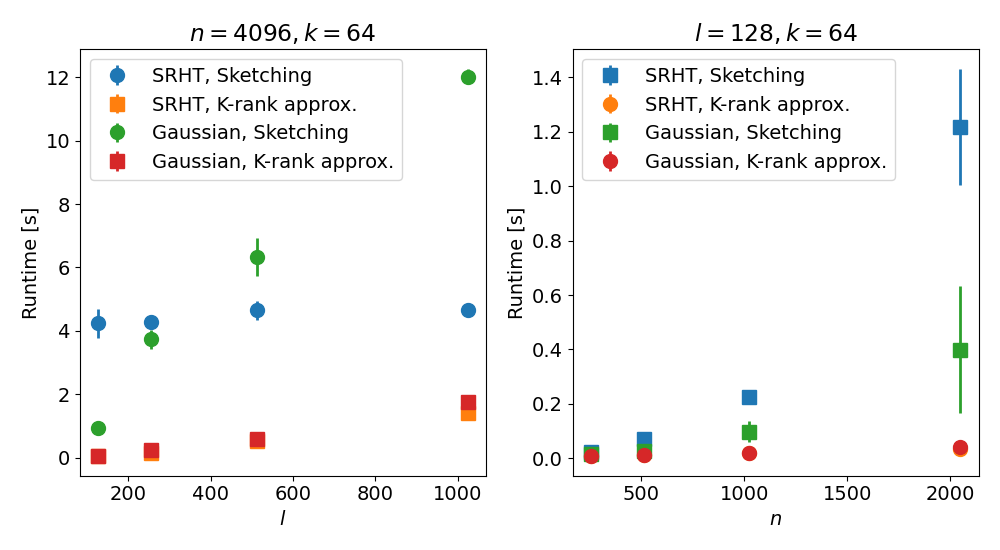
\includegraphics[width=.975\textwidth]{runtimes_l_n_variation}
				\caption{Runtimes associated to the tested sketching methods : as a function of $l$ (left) and as a function of $n$ (right). Runtimes are broken down in that associated to the computation of $A\Omega,\Omega^T A\Omega$ and that associated to the computation of the $k$ rank approximation.}
				\label{fig:runtimes-l-n-variation}
		\end{figure}

		- different behaviours as a function of l and n : as a function of l SRHT looks almost flat, having really slow increase, while gaussian increases steadily given its complexity is or order $nl^2 + ln^2$. This gives advantage for SRHT if we are embedding "dense spaces" as it scales much better than gaussian as function of l. For n : both algos show significant increase, but SRHT shows faster runtime growth. This makes sense due to extra $\log_2(n)$ term in its complexity. This would give advantage to gaussian sketching if we are dealing with sparse information within really high dimensional spaces.
		- 
        \subsection{Parallel Performance}
		- selected $l=n/64$ given we are using TSQR for the QR factorisation and we need the matrix to be tall-skinny to actually observe a speed-up. To have a good speed-up for a bigger $l$, while keeping numerical stability for ill-conditionned matrices another algo should be used.

		- for small example : some speed-up is observed as a function of number of cores but communication costs are non neglectable and even dominate the total runtime for p=64. This is expected as the computation is rather small to be run in parallel. The runtimes for the k-rank are the most affected as these represented the smallest part of the computation to start with. for the specific values selected the gaussian sketching is faster (indeed $l$ is taken only as a small fraction of $n$).

		\begin{figure}[htb]       
			\centering             
				\vspace{0em}
				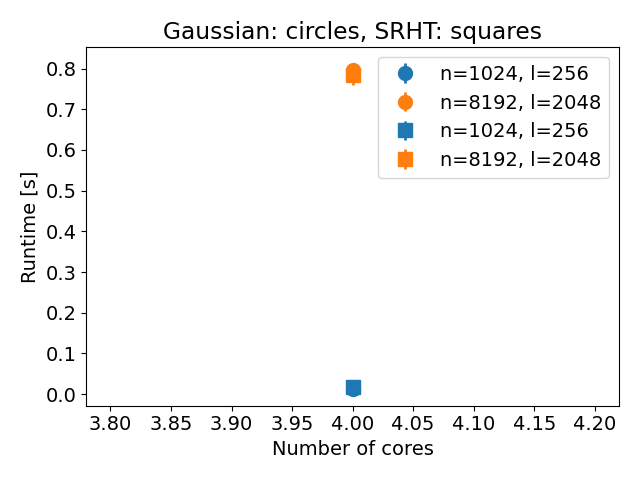
\includegraphics[width=.975\textwidth]{runtimes_cores_variation}
				\caption{Runtimes associated to the tested sketching methods as a function of the number of cores : for a ``small'' example (left) and a ``large'' one (right). Runtimes are broken down in that associated to the computation of $A\Omega,\Omega^T A\Omega$ and that associated to the computation of the $k$ rank approximation.}
				\label{fig:runtimes-cores-variation}
		\end{figure}
		- for the large : communication is not much of an issue, and big speed ups (quasi linear) are observed for the sketching computation. This means the parallelization is successful and scales well for big computations. We can see the speedup is not as good for k-rank partly because the computation was smaller to start with. The fact that the matrix is not that tall-skinny is also expected to have contributed to the low speed-up of that part.
		- 

	\section{Conclusion}
	\section*{Aknowledegments}
	\section*{References}
	%\appendix
	%	\section{Runtime Estimation}\label{appendix:runtime_estimation}
%%%
\end{document} 

